
\de{ĐỀ THI HỌC KỲ I NĂM HỌC 2022-2023}{THPT Thủ Đức}


\Opensolutionfile{ans}[ans/ans]

%Câu 1...........................
\begin{ex}%[0H5B2-3]
Cho tam giác $A B C$ và điểm $M$ thỏa mãn $|\overrightarrow{MB}-\overrightarrow{MC}|=|\overrightarrow{BM}-\overrightarrow{BA}|$. Tập hợp điểm $M$ là	
	\choice
	{Đường trung trực của đoạn $BC$}
	{Đường thẳng $AB$}
	{\True Đường tròn tâm $A$ bán kính $BC$}
	{Đường thẳng qua $A$ và song song với $BC$}
	\loigiai{
		$|\overrightarrow{MB}-\overrightarrow{MC}|=|\overrightarrow{BM}-\overrightarrow{BA}|\Leftrightarrow |\vec{CB}|=|\vec{AM}|\Rightarrow CB=AM$.\\
		Vậy tập hợp điểm $M$ là đường tròn tâm $A$, bán kính $BC$.
	}
\end{ex}
%Câu 2...........................
\begin{ex}%[0H4Y3-1]
	Cho tam giác $ABC$, đặt $AB=c, AC=b, BC=a$. Gọi $R, r$ và $p$ lần lượt là bán kính đường tròn ngoại tiếp, đường tròn nội tiếp và nửa chu vi $\triangle ABC$. Kí hiệu $S$ là diện tích $\triangle A B C$. Hệ thức nào sau đây \textbf{sai}?
	\choice
	{$c=2 R \cdot \sin C$}
	{$p=\dfrac{S}{r}$}
	{$c^2=a^2+b^2-2 a b \cos C$}
	{\True $S=\dfrac{a b c}{4 r}$}
	\loigiai{
		Ta có $S=\dfrac{a b c}{4R}$ nên $S=\dfrac{a b c}{4 r}$ là đáp án sai.
	}
\end{ex}
%Câu 3...........................
\begin{ex}%[0D3Y1-1]
	Cho hàm số $f(x)=\heva{&x^2+3x \text { khi } x \geq 0\\&3-x \text { khi } x<0}$. Giá trị của $f(-1)$ bằng
	\choice
	{$5$}
	{$2$}
	{\True $4$}
	{$-2$}
	\loigiai{
	Ta có	$f(-1)=3-(-1)=4$.
	}
\end{ex}
%Câu 4...........................
\begin{ex}%[0D3Y2-3]
	\immini{Hàm số bậc hai nào trong các hàm số sau có đồ thị như hình vẽ dưới đây?
	\choice
	{$y=x^2-4x$}
	{$y=x^2-4x+4$}
	{$y=-x^2+4x+4$}
	{\True $y=-x^2+4x$}}
{\begin{tikzpicture}[scale=0.6, font=\footnotesize,line join=round, line cap=round, >=stealth];
		\draw[->] (-1.5,0)--(5,0) node[below left ] {$x$};
		\draw[->] (0,-1)--(0,5) node[below left] {$y$};
		\draw (0,0) node [below left] {$O$}  ;
		\draw[dashed] (0,4)node[left]{$ 4 $}--(2,4)--(2,0)node[below]{$ 2 $};
		\fill (2,4) circle (1pt);
		\foreach \x in {}
		\draw[thin] (\x,1pt)--(\x,-1pt) node [below] {$\x$};
		\foreach \y in {}
		\draw[thin] (1pt,\y)--(-1pt,\y) node [left] {$\y$};		
		\begin{scope}
			\clip (-2.5,-2.5) rectangle (5,4.5);
			\draw[samples=200,domain=-0.2:4.2,smooth,variable=\x] plot (\x,{-1*(\x)^2+4*(\x)});
		\end{scope}
\end{tikzpicture}	}
	\loigiai{
		\begin{itemize}
			\item Vì bề lõm của đồ thị quay xuống nên $a<0\Rightarrow a=-1$.
			\item Đồ thị cắt trục tung tại điểm có tung độ bằng $0\Rightarrow c=0$.
		\end{itemize}
	}
\end{ex}
%Câu 5...........................
\begin{ex}%[0D3B2-1]
	Hàm số nào có bảng biến thiên như trong hình vẽ?
	\choice
	{$y=x^2-2x+5$}
	{$y=2 x^2-8x+5$}
	{\True $y=(x-2)^2+1$}
	{$y=-x^2+4 x+5$}	
	\begin{center}
		
\begin{tikzpicture}
			\tkzTabInit[espcl=2.5,lgt=1.5,nocadre=false]
			{$x$/1,$y$/2.1}
			{$-\infty$,$2$,$+\infty$}
			\tkzTabVar{+/$+\infty$,-/$1$,+/$+\infty$}
		\end{tikzpicture}
	\end{center}
\loigiai{	
	\begin{itemize}
		\item Thay $x=2$ vào $y=x^2-2x+5$, ta có $y=5$.
		\item Thay $x=2$ vào $y=2x^2-8x+5$, ta có $y=-3$.
		\item Thay $x=2$ vào $y=(x-2)^2+1$, ta có $y=1$.
		\item Thay $x=2$ vào $y=2x^2-8x+5$, ta có $y=9$.
	\end{itemize}
	}
\end{ex}
%Câu 6...........................
\begin{ex}%[0D1Y3-1]
	Cho hai tập hợp $M=[-3 ; 6)$ và $N=(0 ; 7]$. Tìm $M \cap N$.
	\choice
	{$M \cap N=(-3 ; 7]$}
	{$M \cap N=[0 ; 7]$}
	{$M \cap N=[-3 ; 0)$}
	{\True $M \cap N=(0 ; 6)$}
	\loigiai{
		Ta có
		\begin{center}
			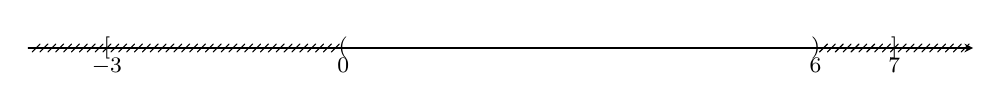
\begin{tikzpicture}[line join = round, line cap = round,>=stealth,font=\footnotesize,scale=1]
				\draw[-stealth] (-4,0)--(8,0);
				\path
				(-3,0) node{$[$} node[below=.05]{$-3$}
				(6,0) node{$)$} node[below=.05]{$6$}
				(0,0) node{$($} node [below=.05]{$0$}
				(7,0) node{$]$} node [below=.05]{$7$}
				;
			\foreach \x in {-3.9,-3.8,...,-3.1}{
				\draw (\x-.05,-.05)--(\x+.05,.05);	
			}
			\foreach \x in {6.1,6.2,...,7.9}{
				\draw (\x-.05,-.05)--(\x+.05,.05);	
		}
		\foreach \x in {-.1,-.2,...,-3}{
			\draw (\x-.05,-.05)--(\x+.05,.05);	
		}
			\end{tikzpicture}
		\end{center}
	Vậy $M \cap N=(0 ; 6)$.
	}
\end{ex}
%Câu 7...........................
\begin{ex}%[0D1B1-3]
	 Phủ định của mệnh đề "$\forall n \in \mathbb{N}, n(n+1)$ là số chẵn" là
	\choice
	{$\exists n \in \mathbb{N}, n(n+1)$ là số chẵn}
	{$\forall n \in \mathbb{N}, n(n+1)$ không là số chẵn}
	{$\exists n \in \mathbb{N}, n(n+1)$ không là số lẻ}
	{\True $\exists n \in \mathbb{N}, n(n+1)$ là số lẻ}
	\loigiai{
		Phủ định của mệnh đề \lq\lq$\forall n \in \mathbb{N}, n(n+1)$ là số chẵn\rq\rq\ là \lq\lq$\exists n \in \mathbb{N}, n(n+1)$ là số lẻ\rq\rq.
	}
\end{ex}
%Câu 8...........................
\begin{ex}%[0H5K2-5]
	Một vật có khối lượng $m$ được treo cố định trên trần nhà bằng 2 sợi dây không dãn có độ đài bằng nhau. Biết rằng lực căng dây $\vec{T}_1$ và $\vec{T}_2$ có độ lớn bằng nhau bằng $600$ N và hợp với nhau một góc $60^{\circ}$ như hình vẽ bên dưới.
	\begin{center}
		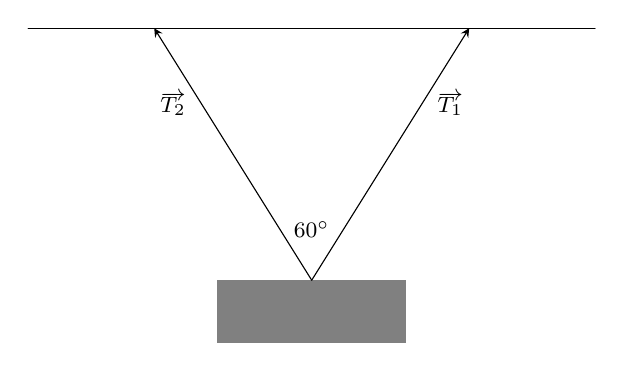
\begin{tikzpicture}[scale=0.8, font=\footnotesize,line join=round, line cap=round, >=stealth];
		%	\draw[thin,opacity=.5] (0,0) grid (9,9);
			\fill[color=gray] (0,0) rectangle (3,1);
			\draw (-3,5)--(6,5);
			\draw[->] (1.5,1)--(-1,5);
			\draw[->](1.5,1)--(4,5);
			\draw (1.5,1.8) node{$60^\circ$} (-0.7,3.8) node{$\overrightarrow{T_2}$} (3.7,3.8) node{$\overrightarrow{T_1}$};	
		\end{tikzpicture}
	\end{center}
	Độ lớn hợp lực của 2 lực căng dây $\vec{T}_1$ và $\vec{T}_2$ là
	\choice
	{$1\,200 \sqrt{3}$ N}
	{\True $600 \sqrt{3}$ N}
	{$1\,200$ N}
	{$600$ N}
	\loigiai{
		\immini
		{
			Ta có $\begin{aligned}[t]
				\left|\vec{T}\right|^2=\vec{T}^2&=\left(\vec{T_1}+\vec{T_2}\right)^2\\
				&=\vec{T_1}^2+\vec{T_2}^2+2\vec{T_1}\cdot\vec{T_2}\\
				&=\vec{T_1}^2+\vec{T_2}^2+2\left|\vec{T_1}\right|\cdot\left|\vec{T_1}\right|\cdot\cos\left(\vec{T_1};\vec{T_2}\right)\\
				&=600^2+600^2+2\cdot600\cdot600\cdot\cos60^\circ\\
				&=1\,080\,000\\
				&\Rightarrow \left|\vec{T}\right|=\sqrt{1\,080\,000}=600\sqrt{3} \mbox{ (N)}.
			\end{aligned}$
		}
		{
			\begin{tikzpicture}[scale=0.8, font=\footnotesize,line join=round, line cap=round, >=stealth,scale=.6];
				%	\draw[thin,opacity=.5] (0,0) grid (9,9);
				\fill[color=gray] (0,0) rectangle (3,1);
				\draw (-3,5)--(6,5);
				\draw[->] (1.5,1) coordinate (B)--(-1,5) coordinate (a);
				\draw[->](1.5,1)--(4,5) coordinate (b);
				\draw[->] (B)--($(a)!.5!(b)$) coordinate (c)--($(B)!2!(c)$) coordinate (A) node[above]{$\vec{T}$};
				\draw[dashed]
				(-1,5)--(A)
				;
				\draw[dashed]
				(4,5)--(A) 
				;
				\draw (-1.2,3.8) node{$\overrightarrow{T_2}$} (4,3.8) node{$\overrightarrow{T_1}$};	
			\end{tikzpicture}
		}
	}
\end{ex}
%Câu 9...........................
\begin{ex}%[0H5B4-3]
	Cho hình chữ nhật $ABCD$ tâm là $O, AD=3$ và $AB=5$. Gọi $M$ là điểm thỏa mãn $\overrightarrow{AM}=m \overrightarrow{AB}$ với $m \in \mathbb{R}$. Tìm $m$ để $\triangle AOM$ vuông tại $O$.
	\choice
	{\True $m=\dfrac{17}{25}$}
	{$m=\dfrac{17}{15}$}
	{$m=\dfrac{17}{9}$}
	{$m=\dfrac{13}{20}$}
	\loigiai{
		\immini
		{
			Ta có
			\begin{itemize}
				\item Vì $ABCD$ là hình chữ nhật nên $\vec{AB}\cdot\vec{AD}=0$.
				\item $\vec{AO}=\dfrac{1}{2}\left(\vec{AD}+\vec{AB}\right)=\dfrac{1}{2}\vec{AD}+\dfrac{1}{2}\vec{AB}$.
				\item $\vec{AM}=m\vec{AB}$.
				\item $\begin{aligned}[t]
					\vec{OM}=\vec{AM}-\vec{AO}&=m\vec{AB}-\dfrac{1}{2}\vec{AD}-\dfrac{1}{2}\vec{AB}\\
					&=\left(m-\dfrac{1}{2}\right)\vec{AB}-\dfrac{1}{2}\vec{AD}.
				\end{aligned}$
			\item $\begin{aligned}[t]
				\vec{OA}\cdot\vec{OM}&=\left(-\dfrac{1}{2}\vec{AB}-\dfrac{1}{2}\vec{AD}\right)\cdot\left[\left(m-\dfrac{1}{2}\right)\vec{AB}-\dfrac{1}{2}\vec{AD}\right]\\
				&=-\dfrac{1}{2}\left(m-\dfrac{1}{2}\right)\vec{AB}^2+\dfrac{1}{4}\vec{AD}^2\\
				&=-\dfrac{1}{2}\left(m-\dfrac{1}{2}\right)\cdot5^2+\dfrac{1}{4}\cdot3^2\\
				&=-\dfrac{25}{2}m+\dfrac{25}{4}+\dfrac{9}{4}\\
				&=-\dfrac{25}{2}m+\dfrac{17}{2}.
			\end{aligned}$
		\item Vì $\triangle AOM$ vuông tại $O$ nên
		$\begin{aligned}[t]
			&\vec{OA}\cdot\vec{OM}=0\\
			&\Rightarrow-\dfrac{25}{2}m+\dfrac{17}{2}=0\\
			&\Leftrightarrow-\dfrac{25}{2}m=-\dfrac{17}{2}\\
			&\Leftrightarrow m=\dfrac{17}{25}.
		\end{aligned}$
			\end{itemize}
		}
		{
			\begin{tikzpicture}[line join = round, line cap = round,>=stealth,font=\footnotesize,scale=1]
				\draw
				(0,0) coordinate (A) -- (5,0) coordinate (B) -- (5,3) coordinate (C) -- (0,3) coordinate (D)--cycle
				(17/5,0) coordinate (M)
				(A)--(C) (B)--(D)
				($(A)!.5!(C)$) coordinate (O)--(M)
				;
				\foreach \x/\g in {A/180,B/0,C/0,D/180,M/-90,O/90} \fill (\x) circle (1.5pt) ($(\x)+(\g:3mm)$) node{$\x$};
			\end{tikzpicture}
		}
	}
\end{ex}
%Câu 10...........................
\begin{ex}%[0D3K2-5]
	Một vận động viên ném một quả bóng vào rổ. Rổ ở độ cao $3{,}05$ m và cách vận động viên $7$ m theo phương ngang. Quả bóng rời tay vận động viên ở độ cao $2{,}1$ m và có tốc độ là $v$ (m/s). Nếu gốc tọa độ được đặt tại chân vận động viên thì quỹ đạo của quả bóng khi rời tay vận động viên là một đường cong cho bởi hàm số sau $y=-\dfrac{10}{v^2} \cdot x^2+x+2{,}1$, trong đó $x$ là quãng đường tính bằng mét mà bóng đi được theo phương ngang (tham khảo hình vẽ bên dưới) và $y$ là độ cao của quả bóng tính bằng mét.
	\begin{center}
		\begin{tikzpicture}[scale=1.0, font=\footnotesize,line join=round, line cap=round, >=stealth];			
			\draw[->] (0,0)--(8,0) node[below left ] {$x$};
			\draw[->] (0,0)--(0,4) node[below left] {$y$};
			\draw (0,0) node [below left] {$O$}  ;
			\draw[dashed,<->] (7,0)--(7,39/16)node [right] {Rổ};
			\draw (-0.2,2)node [left] {$2{,}1\,m$};
			\draw (7,0)node [below] {$7\,m$};
			\draw (7,1.5)node [right] {$3{,}05\,m$};			
			\foreach \x in {}
			\draw[thin] (\x,1pt)--(\x,-1pt) node [below] {$\x$};
			\foreach \y in {}
			\draw[thin] (1pt,\y)--(-1pt,\y) node [left] {$\y$};		
			\draw[name path=c1,smooth, samples=300, domain=0:7] plot (\x,{-1/16*(\x)^2+1/2*(\x)+2});
			\fill[blue] (0,2) circle (7pt);
		\end{tikzpicture}
	\end{center}
	Biết vận động viên ghi được điểm. Tìm độ cao lớn nhất mà bóng có thể đạt được (làm tròn đến 1 số thập phân sau dấu phẩy).
	\choice
	{\True $4{,}1$ m}
	{$3{,}5$ m}
	{$4{,}5$ m}
	{$5{,}2$ m}
	\loigiai{
		Thay $x=7$ và $y=3{,}05$ vào $y=-\dfrac{10}{v^2} \cdot x^2+x+2{,}1$, ta có
		\[
		3{,}05=-\dfrac{10}{v^2} \cdot 7^2+7+2{,}1\Leftrightarrow-\dfrac{10}{v^2} \cdot 49=\dfrac{-121}{20}\Leftrightarrow -\dfrac{10}{v^2}=\dfrac{-121}{980}.
		\]
		Do đó $y=-\dfrac{121}{980} \cdot x^2+x+2{,}1$.\\
Vậy độ cao lớn nhất mà bóng có thể đạt được chính là tung độ của đỉnh $S$ của hàm số $y=-\dfrac{121}{980} \cdot x^2+x+2{,}1\Rightarrow y_S=\dfrac{-\Delta}{4a}=\dfrac{-1^2+4\cdot\left(-\dfrac{121}{980}\right)\cdot2{,}1}{4\cdot\left(-\dfrac{121}{980}\right)}\approx4{,}1$.
	}
\end{ex}

%Câu 11...........................
\begin{ex}%[0T3B2-1]%[Dự án đề kiểm tra HKI NH22-23- PHẠM VĂN LONG]%[TRƯỜNG THPT THỦ ĐỨC]
	Đồ thị hàm số $y=-x^2-4 x+2022$ có đỉnh là
	\choice
	{$I(2 ;-2026)$}
	{$I(-2 ;-2026)$}
	{\True $I(-2 ;2026)$}
	{$I(2 ;2026)$}
	\loigiai{
	Đồ thị hàm số $y=-x^2-4 x+2022$ có đỉnh $I(-2 ;2026)$.	
	}
\end{ex}
%Câu 12...........................
\begin{ex}%[0T3B1-2]%[Dự án đề kiểm tra HKI NH22-23- PHẠM VĂN LONG]%[TRƯỜNG THPT THỦ ĐỨC]
	Tập xác định của hàm số $y=\sqrt{x+1}+\dfrac{x+2}{x}$ là
	\choice
	{$(-1 ;+\infty)\setminus \{0\}$}
	{$\mathbb{R} \setminus\{0\}$}
	{$(-1 ;+\infty)$}
	{\True $[-1 ;+\infty) \setminus\{0\}$}
	\loigiai{
	Diều kiện $\heva{&x+1\ge 0\\&x\ne 0}\Leftrightarrow \heva{&x\ge -1\\&x\ne 0.}$\\	
	Vậy $\mathscr{D}=[-1 ;+\infty) \setminus\{0\}$.
	}
\end{ex}
%Câu 13...........................
\begin{ex}%[0T4B3-1]%[Dự án đề kiểm tra HKI NH22-23- PHẠM VĂN LONG]%[TRƯỜNG THPT THỦ ĐỨC]
	Cho tam giác $A B C$ có $A B=6, B C=8$, $\widehat{A B C}=120^{\circ}$. Diện tích $S$ tam giác $A B C$ bằng
	\choice
	{$13{,}9$}
	{\True $12 \sqrt{3}$}
	{$24 \sqrt{3}$}
	{$21$}
	\loigiai{
	Ta có $S_{\triangle ABC}=\dfrac{1}{2}\cdot AB\cdot BC\cdot \sin B=\dfrac{1}{2}\cdot 6\cdot 8\cdot \sin 120^\circ=12 \sqrt{3}$.	
	}
\end{ex}
%Câu 14...........................
\begin{ex}%[0T3B2-3]%[Dự án đề kiểm tra HKI NH22-23- PHẠM VĂN LONG]%[TRƯỜNG THPT THỦ ĐỨC]
	Tìm $m$ để đồ thị hàm số $y=x^2-(m+1) x+4 m-5$ nhận $x=2$ là trục đối xứng.
	\choice
	{$m=1$}
	{$m=-3$}
	{\True $m=3$}
	{$m=-5$}
	\loigiai{
	Đồ thị hàm số $y=x^2-(m+1) x+4 m-5$ nhận $x=2$ là trục đối xứng	suy ra	
	$$\dfrac{m+1}{2}=2\Leftrightarrow m=3.$$
	}
\end{ex}
%Câu 15...........................
\begin{ex}%[0T1B2-1]%[Dự án đề kiểm tra HKI NH22-23- PHẠM VĂN LONG]%[TRƯỜNG THPT THỦ ĐỨC]
	Trong các tập hợp sau tập hợp nào có hai phần tử? 
	\choice
	{$\left\{x \in \mathbb{R} \middle | x^2-x+6=0\right\}$}
	{$\left\{x \in \mathbb{Z} \middle | 2 x^2-5 x+2=0\right\}$}
	{\True $\left\{n \in \mathbb{N} \middle | n^2 \leq 1\right\}$}	
	{$\left\{n \in \mathbb{N} \middle | n \leq 2\right\}$}
	\loigiai{
		\begin{itemize}
			\item Ta có $x^2-x+6=0$ vô nghiệm.
			\item Ta có $2 x^2-5 x+2=0\Leftrightarrow \hoac{&x=2\text{ (thỏa)}\\&x=\dfrac{1}{2} \text{ (loại).}}$
			\item Ta có $n^2 \leq 1$ và $n \in \mathbb{N} \Rightarrow n\in \{0;2\}$.
			\item Ta có $n \leq 2$ và $n \in \mathbb{N} \Rightarrow n\in \{0;1;2\}$.
		\end{itemize}	
	}
\end{ex}
%Câu 16...........................
\begin{ex}%[0T3B2-2]%[Dự án đề kiểm tra HKI NH22-23- PHẠM VĂN LONG]%[TRƯỜNG THPT THỦ ĐỨC]
	Hàm số $y=x^2-4 x+11$ nghịch biến trên khoảng
	\choice
	{$(2 ;+\infty)$}
	{$(7 ;+\infty)$}
	{\True $(-\infty ; 2)$}
	{$(4 ;+\infty)$}
	\loigiai{
		Hàm số $y=x^2-4 x+11$ nghịch biến trên khoảng $(-\infty ; 2)$ và đồng biến trên khoảng $(2;+\infty)$.
	}
\end{ex}
%Câu 17...........................
\begin{ex}%[0T3B2-1]%[Dự án đề kiểm tra HKI NH22-23- PHẠM VĂN LONG]%[TRƯỜNG THPT THỦ ĐỨC]
	Tìm tất cả các giá trị của tham số $m$ để hàm số $y=\left(m^2-1\right) x^3+(m+1) x^2+5 x-3$ là hàm số bậc hai.
	\choice
	{$m \neq \pm 1$}
	{$m \neq-1$}
	{\True $m=1$}
	{$m \in \mathbb{R}$}
	\loigiai{
	Hàm số $y=\left(m^2-1\right) x^3+(m+1) x^2+5 x-3$ là hàm số bậc hai khi\\
	$$\heva{&m^2-1= 0\\&m+1\ne 0}\Leftrightarrow m=1.$$	
	}
\end{ex}
%Câu 18...........................
\begin{ex}%[0T5B2-2] %[Dự án đề kiểm tra HKI NH22-23- PHẠM VĂN LONG]%[TRƯỜNG THPT THỦ ĐỨC]
	Cho ba điểm $A, B, C$ phân biệt thỏa mãn $3 \overrightarrow{O C}=2 \overrightarrow{O A}+\overrightarrow{O B}$ với mọi điểm $O$. Mệnh đề nào sau đây là đúng?
	\choice
	{\True Ba điểm $A, B, C$ thẳng hàng}
	{Ba điểm $A, B, C$ tạo thành tam giác vuông}
	{Ba điểm $A, B, C$ tao thành tam giác cân}
	{$C$ là trung điểm của $A B$}
	\loigiai{
	Ta có $3 \overrightarrow{O C}=2 \overrightarrow{O A}+\overrightarrow{O B}\Leftrightarrow 2\left(\overrightarrow{OC}-\overrightarrow{O A}\right)=\left(\overrightarrow{OB}-\overrightarrow{OC}\right)\Leftrightarrow 2\overrightarrow{AC}=\overrightarrow{CB}$.\\
	Suy ra ba điểm $A, B, C$ thẳng hàng.
	}
\end{ex}
%Câu 19...........................
\begin{ex}%[0T5B2-2] %[Dự án đề kiểm tra HKI NH22-23- PHẠM VĂN LONG]%[TRƯỜNG THPT THỦ ĐỨC]
	Khẳng định nào sau đây là \textbf{sai}?
	\choice
	{Nếu $G$ là trọng tâm của tam giác $A B C$ thì $\overrightarrow{G A}+\overrightarrow{G B}=\overrightarrow{C G}$}
	{Với 3 điểm $I, J, K$ bất kỳ ta có $\overline{I J}+\overrightarrow{J K}=\overrightarrow{I K}$}
	{\True Nếu $\overrightarrow{A B}+\overrightarrow{A D}=\overrightarrow{A C}$ thì $A B C D$ là hình bình hành}
	{Nếu $I$ là trung điểm của $A B$ thì với mọi điểm $M$ ta có $\overrightarrow{M A}+\overrightarrow{M B}=2 \overrightarrow{M I}$}
	\loigiai{
	Nếu $\overrightarrow{A B}+\overrightarrow{A D}=\overrightarrow{A C}$ thì $A B C D$ là hình bình hành là đáp án \textbf{sai}  khi $A,B,C,D$ thẳng hàng.
	}
\end{ex}
%Câu 20...........................
\begin{ex}%[0T5B2-2] %[Dự án đề kiểm tra HKI NH22-23- PHẠM VĂN LONG]%[TRƯỜNG THPT THỦ ĐỨC]
	Cho các điểm $A, B$, $O$. Khẳng định nào sau đây là đúng?
	\choice
	{$\overrightarrow{A B}=\overrightarrow{O A}+\overrightarrow{O B}$}
	{\True $\overrightarrow{A B}=\overrightarrow{O B}-\overrightarrow{O A}$}
	{$\overline{A B}=\overrightarrow{O A}-\overrightarrow{O B}$}
	{$\overrightarrow{A B}=\overrightarrow{A O}-\overrightarrow{O B}$}
	\loigiai{
	Ta có $\overrightarrow{O B}-\overrightarrow{O A}=\overrightarrow{A B}$.
	}
\end{ex}


%Câu 21...........................
\begin{ex}%[Đề thi HK1, THPT Thủ Đức TPHCM 2022-2023]%[0H5B4-1]
	Cho hình vuông $ABCD$ có độ dài cạnh bằng $10$. Tính giá trị $\overrightarrow{AB} \cdot \overrightarrow{CD}$
	\choice
	{$100$}
	{$10$}
	{$0$}
	{\True $-100$}
	\loigiai{
	Vì $\overrightarrow{CD}=-\overrightarrow{AB}$ nên 	$\overrightarrow{AB} \cdot \overrightarrow{CD}=-\overrightarrow{AB}^2=-100$.
	}
\end{ex}
%Câu 22...........................
\begin{ex}%[Đề thi HK1, THPT Thủ Đức TPHCM 2022-2023]%[0H5B2-1]
	Cho $4$ điểm phân biệt $A, B, C, D$. Thu gọn $\overrightarrow{u}=\overrightarrow{AD}-\overrightarrow{AB}-\overrightarrow{BC}-\overrightarrow{CA}$ ta được kết quả là
	\choice
	{$\overrightarrow{u}=\overrightarrow{0}$}
	{$\overrightarrow{u}=\overrightarrow{CD}$}
	{$\overrightarrow{u}=\overrightarrow{DB}$}
	{\True $\overrightarrow{u}=\overrightarrow{AD}$}
	\loigiai{
Ta có $\overrightarrow{u}=\left(\overrightarrow{AD}-\overrightarrow{AB}\right)-\left(\overrightarrow{BC}+\overrightarrow{CA}\right)=\overrightarrow{BD}-\overrightarrow{BA}=\overrightarrow{AD}$.		
	}
\end{ex}
%Câu 23...........................
\begin{ex}%[Đề thi HK1, THPT Thủ Đức TPHCM 2022-2023]%[0D2B2-1]
	Cho hệ bất phương trình $\heva{&x-y<3\\&x+2y\ge-2}$. Điểm nào sau đây thuộc miền nghiệm của hệ bất phương trình đã cho?
	\choice
	{$(3 ; 0)$}
	{\True $(1 ; 0)$}
	{$(2 ;-1)$}
	{$(-2 ;-3)$}
	\loigiai{
Vì $\heva{& 1-0<3 \\ & 1+2\cdot 0\ge -2}$ nên điểm $(1;0)$ thuộc miền nghiệm của hệ bất phương trình đã cho.		
	}
\end{ex}
%Câu 24...........................
\begin{ex}%[Đề thi HK1, THPT Thủ Đức TPHCM 2022-2023]%[0D3B2-3]
	Tìm $a$ để hàm số $y=-x^2+2x+3-2a$ đạt giá trị lớn nhất bằng $2022$.
	\choice
	{$a=-1001$}
	{$a=1009$}
	{\True $a=-1009$}
	{$a=1001$}
	\loigiai{
Ta có $y=-(x^2-2x+1)+4-2a=-(x-1)^2+4-2a\le 4-2a$.\\
Theo yêu cầu bài toán, để hàm số đạt giá trị lớn nhất bằng $2022$ khi và chỉ khi
$$4-2a=2022\Leftrightarrow a=-1009.$$		
	}
\end{ex}
%Câu 25...........................
\begin{ex}%[Đề thi HK1, THPT Thủ Đức TPHCM 2022-2023]%[0D3B1-4]
	\immini{Cho hàm số $f(x)$ với tập xác định là đoạn $[-1 ; 4]$ có đồ thị như hình vẽ bên dưới.
	Khẳng định nào sau đây là \textbf{sai}?
	\choice
	{\True Hàm số $f(x)$ đạt giá trị lớn nhất là $3$}
	{Hàm số $f(x)$ đồng biến trên khoảng $(2 ; 4)$}
	{Hàm số $f(x)$ đạt giá trị nhỏ nhất là $-1$}
	{Hàm số $f(x)$ nghịch biến trên khoảng $(1 ; 2)$}}
	{\begin{tikzpicture}[scale=0.8, font=\footnotesize, line join=round, line cap=round, >=stealth]
			\draw [->] (-2,0)--(5,0) node[below]{$x$};
			\draw [->] (0,-2)--(0,5) node[right]{$y$};
			\draw[fill=black] (0,0) circle(1pt) node[below left]{$O$};
			%%\draw[opacity=0.1] (-3,-3) grid (10,7);
			%\clip (-5,-3) rectangle (11,8);
			\draw[name path=c1,smooth, samples=300, domain=-1:2] plot (\x,{-1*(\x)^2+2*(\x)+2});
			\draw (2,2)--(4,4);
			\draw[dashed] (1,0)--(1,3)--(0,3);
			\draw[dashed] (-1,0)--(-1,-1)--(0,-1);
			\draw[dashed] (4,0)--(4,4)--(0,4);
			\draw[dashed] (2,0)--(2,2)--(0,2);
			\draw [fill=black] (-1,-1) circle(1pt);
			\draw [fill=black](1,3) circle(1pt);
			\draw [fill=black](4,4) circle(1pt);
			\draw [fill=black] (-1,0.2) node[left]{$-1$} (0,-1) node[right]{$-1$} (0,2) node[left]{$2$} (0,3) node[left]{$3$} (0,4) node[left]{$4$} (1,0) node[below]{$1$} (2,0) node[below]{$2$} (4,0) node[below]{$4$};			
	\end{tikzpicture}}
	\loigiai{
	Khẳng định sai là \lq\lq Hàm số đạt giá trị lớn nhất là $3$\rq\rq\ .	
	}
\end{ex}
%Câu 26...........................
\begin{ex}%[Đề thi HK1, THPT Thủ Đức TPHCM 2022-2023]%[0H5B3-2]
	Cho ba điểm phân biệt $A, B, C$. Nếu $\overrightarrow{AB}=-3\overrightarrow{BC}$ thì đẳng thức nào dưới đây đúng?
	\choice
	{$\overrightarrow{AC}=2\overrightarrow{BC}$}
	{$AB=-3BC$}
	{$\overrightarrow{AB}+3\overrightarrow{CB}=\overrightarrow{0}$}
	{\True $\overrightarrow{AC}=\dfrac{2}{3}\overrightarrow{AB}$}
	\loigiai{
Ta có 	$\overrightarrow{AB}=-3\overrightarrow{BC}\Leftrightarrow \overrightarrow{AB}=-3\left(\overrightarrow{AC}-\overrightarrow{AB}\right)\Leftrightarrow 3\overrightarrow{AC}=2\overrightarrow{AB}\Leftrightarrow \overrightarrow{AC}=\dfrac{2}{3}\overrightarrow{AB}$.
	}
\end{ex}
%Câu 27...........................
\begin{ex}%[Đề thi HK1, THPT Thủ Đức TPHCM 2022-2023]%[0D3Y1-2]
	Tập xác định của hàm số $y=\dfrac{x+1}{x^2+1}$ là
	\choice
	{\True $\mathbb{R}$}
	{$\mathbb{R} \setminus \{-1\}$}
	{$\mathbb{R} \setminus \{\pm 1\}$}
	{$(-1;+\infty)$}
	\loigiai{
Vì $x^2+1>0$ với mọi $x\in\mathbb{R}$ nên tập xác định của hàm số là $\mathbb{R}$.		
	}
\end{ex}
%Câu 28...........................
\begin{ex}%[Đề thi HK1, THPT Thủ Đức TPHCM 2022-2023]%[0H5B1-2]
	\immini{Cho hình bình $ABCD$ có tâm $O$. Các cặp véc-tơ nào sau đây là véc-tơ đối nhau?
	\choice
	{$\overrightarrow{AD}$ và $\overrightarrow{BC}$}
	{$\overrightarrow{OD}$ và $\overrightarrow{BO}$}
	{$\overrightarrow{CD}$ và $\overrightarrow{BA}$}
	{\True $\overrightarrow{AO}$ và $\overrightarrow{CO}$}}
{\begin{tikzpicture}[>=stealth,smooth,line join=round,line cap=round,font=\footnotesize,scale=0.7]	
		\path
		(0,0) coordinate (A)
		(4,0) coordinate (B)
		(5,2) coordinate (C)
		(1,2) coordinate (D)
		($(A)!0.5!(C)$) coordinate (O);
		\draw (A)--(B)--(C)--(D)--(A)--(C) (B)--(D); 
		\foreach \x/\g in {A/180,B/0,C/90,D/90,O/90} \fill[black] (\x) circle (1pt)+(\g:3mm) node{$\x$};
\end{tikzpicture}}
	\loigiai{
Cặp véc-tơ đối nhau là $\overrightarrow{AO}$ và $\overrightarrow{CO}$.		
	}
\end{ex}
%Câu 29...........................
\begin{ex}%[Đề thi HK1, THPT Thủ Đức TPHCM 2022-2023]%[0H5B3-4]
	Cho hình bình hành $ABCD$. Gọi $M$ là trung điểm của cạnh $AD$. Trên cạnh $BC$ lấy điểm $N$ sao cho $BC=3BN$. Chọn khẳng định đúng.	
	\choice
	{$\overrightarrow{MN}=\dfrac{2}{3} \overrightarrow{AB}-\dfrac{1}{2} \overrightarrow{AD}$}
	{\True $\overrightarrow{MN}=\overrightarrow{AB}-\dfrac{1}{6} \overrightarrow{AD}$}
	{$\overrightarrow{MN}=\dfrac{1}{6} \overrightarrow{AB}-\overrightarrow{AD}$}
	{$\overrightarrow{MN}=\dfrac{1}{2} \overrightarrow{AB}-\dfrac{1}{3} \overrightarrow{AD}$}
	\loigiai{
\immini
{
Ta có 
\begin{eqnarray*}
	\overrightarrow{MN}&=&  \overrightarrow{AN}-\overrightarrow{AM}\\
	&=& \overrightarrow{AB}+\overrightarrow{BN}-\dfrac{1}{2}\overrightarrow{AD}\\
	&=& \overrightarrow{AB}+\dfrac{1}{3}\overrightarrow{BC}-\dfrac{1}{2}\overrightarrow{AD}\\
	&=& \overrightarrow{AB}+\dfrac{1}{3}\overrightarrow{AD}-\dfrac{1}{2}\overrightarrow{AD}\\
	&=& \overrightarrow{AB}-\dfrac{1}{6} \overrightarrow{AD}.
\end{eqnarray*}
}
{
\begin{tikzpicture}[>=stealth,smooth,line join=round,line cap=round,font=\footnotesize,scale=1]	
	\path
	(0,0) coordinate (A)
	(4,0) coordinate (B)
	(5,2) coordinate (C)
	(1,2) coordinate (D)
	($(A)!0.5!(D)$) coordinate (M) ($(B)!1/3!(C)$) coordinate (N);
	\draw (A)--(B)--(C)--(D)--(A) (M)--(N); 
	\foreach \x/\g in {A/180,B/0,C/90,D/90,M/180,N/0} \fill[black] (\x) circle (1pt)+(\g:3mm) node{$\x$};
\end{tikzpicture}
}		
	}
\end{ex}
%Câu 30...........................
\begin{ex}%[Đề thi HK1, THPT Thủ Đức TPHCM 2022-2023]%[0D3B2-1]
	Tập giá trị của hàm số $y=7x^2-14x+23$ là
	\choice
	{\True $[16;+\infty)$}
	{$(16;+\infty)$}
	{$[1;+\infty)$}
	{$\mathbb{R}$}
	\loigiai{
Ta có $y=7\left(x^2-2x+1\right)+16=7(x-1)^2+16\ge 16$.\\
Vậy tập giá trị của hàm số là 	$[16;+\infty)$.	
	}
\end{ex}

\begin{ex}%[0T1Y1-1]%[Dự án đề kiểm tra HKI NH22-23- Võ Thị Thùy Trang]%[Thủ Đức]
	Có bao nhiêu phát biểu là mệnh đề?
	\begin{itemize}
		\item Hà Nội là Thủ đô của Việt Nam.
		\item Số 16 là một số chính phương.
		\item $x=1$ có phải là nghiệm của phương trình $x^2-1=0$ không?
		\item Phương trình $3x^2-5x+2=0$ có nghiệm nguyên.
		\item $5<7-3$.
	\end{itemize}
	\choice
	{$3$}
	{$2$}
	{\True $4$}
	{$5$}
	\loigiai{Có $4$ phát biểu là mệnh đề đó là 
		\begin{itemize}
			\item Hà Nội là Thủ đô của Việt Nam.
			\item Số 16 là một số chính phương.
			\item Phương trình $3x^2-5x+2=0$ có nghiệm nguyên.
			\item $5<7-3$.
		\end{itemize}
	}
\end{ex}
\begin{ex}%[0T2Y1-1]%[Dự án đề kiểm tra HKI NH22-23- Võ Thị Thùy Trang]%[Thủ Đức]
	Bất phương trình nào sau đây \textbf{không} phải là bất phương trình bậc nhất hai ẩn?
	\choice
	{\True $(x+3)y+1 \leq 0$}
	{$\dfrac{x}{2}-\dfrac{y}{13}+10<0$}
	{$2x-13y+5<0$}
	{$x-5y-13 \geq 0$}
	\loigiai{Bất phương trình $(x+3)y+1 \leq 0$ không phải là bất phương trình bậc nhất hai ẩn.
	}
\end{ex}
\begin{ex}%[0T5B4-1]%[Dự án đề kiểm tra HKI NH22-23- Võ Thị Thùy Trang]%[Thủ Đức]
	Cho tam giác $ABC$ có $AB=AC=1$, $\widehat{BAC}=120^{\circ}$, $M\in AB$ sao cho $AM=\dfrac{1}{3}$. Khi đó $\overrightarrow{AM} \cdot \overrightarrow{AC}$ bằng
	\choice
	{$\dfrac{1}{2}$}
	{$-\dfrac{3}{8}$}
	{\True $-\dfrac{1}{6}$}
	{$-\dfrac{3}{2}$}
	\loigiai{Ta có $\overrightarrow{AM} \cdot \overrightarrow{AC}=AM\cdot AC\cdot \cos \widehat{MAC}=\dfrac{1}{3}\cdot 1\cdot \cos 120^{\circ}=-\dfrac{1}{6}$.
	}
\end{ex}
\begin{ex}%[0T2K2-1]%[Dự án đề kiểm tra HKI NH22-23- Võ Thị Thùy Trang]%[Thủ Đức]
	\immini{
		Tìm giá trị nhỏ nhất của biểu thức $F(x,y)=10x-30y$ với $(x ; y)$ là nghiệm của hệ bất	phương trinh có miền nghiệm là phần được tô đậm trong hình vẽ bên.
		\choice
		{$-20$}
		{\True $-40$}
		{$-60$}
		{$30$}}
	{\begin{tikzpicture}[scale=.7,>=stealth, font=\footnotesize, line join=round, line cap=round]
			%			\draw[color=gray!50,dashed] (-5,-5) grid (5,5);
			\draw[->] (-4,0)--(5,0) node [below]{$x$};
			\draw[->] (0,-2)--(0,5) node [left]{$y$};
			\node at (0,0) [below left]{$O$};
			\clip (-4,-2) rectangle (5,5);
			\draw[smooth,samples=300] plot(\x,{(1/2)*\x+1});
			\draw[smooth,samples=300] plot(\x,{(-2)*\x+6});
			\fill[pattern=north east lines,opacity=0.8] plot[domain=-2:3](\x,{(1/2)*\x+1})--(2,2)--plot(\x,{(-2)*\x+6})--(3,0)--cycle;
			\node at (-2,0) [above]{$-2$};
			\node at (3,0) [above right]{$3$};
			\draw[dashed] (0,2)node [left]{$2$}--(2,2)--(2,0)node [below]{$2$};
	\end{tikzpicture}}
	\loigiai{Ta có $F(-2,0)=-20$; $F(2,2)=-40$; $F(3,0)=30$. Suy ra giá trị nhỏ nhất của biểu thức $F(x,y)=10x-30y$ là $-40$.
	}
\end{ex}
\begin{ex}%[Dự án đề kiểm tra HKI NH22-23- Võ Thị Thùy Trang]%[Thủ Đức]
	Cho tam giác $ABC$ có $AB=3$, $AC=6$ và $\widehat{BAC}=120^{\circ}$. Giá trị của tích vô hướng $\overrightarrow{AB}\cdot \overrightarrow{AC}$ bằng
	\choice
	{$-9\sqrt{3}$}
	{$9$}
	{$9\sqrt{3}$}
	{\True $-9$}
	\loigiai{Ta có $\overrightarrow{AB} \cdot \overrightarrow{AC}=AB\cdot AC\cdot \cos \widehat{BAC}=3\cdot 6\cdot \cos 120^{\circ}=-9$.
	}
\end{ex}
\begin{ex}%[0T5B3-1]%[Dự án đề kiểm tra HKI NH22-23- Võ Thị Thùy Trang]%[Thủ Đức]
	Cho tam giác $ABC$ đều có trọng tâm $G$. Gọi $M$ là trung diểm của $BC$. Khẳng định nào sau đây là đúng?
	\choice
	{$\overrightarrow{AM}=3\overrightarrow{AG}$}
	{\True $\overrightarrow{GA}=-2\overrightarrow{GM}$}
	{$\overrightarrow{GA}=\overrightarrow{GB}=\overrightarrow{GC}$}
	{$\overrightarrow{M B}=\dfrac{1}{2} \overrightarrow{BC}$}
	\loigiai{\immini{$\overrightarrow{GA}=-2\overrightarrow{GM}$.}
		{\begin{tikzpicture}[scale=0.7, font=\footnotesize, line join=round, line cap=round, >=stealth]
				\def\bc{4} % cạnh BC
				\def\ba{4} % cạnh BA
				\def\h{4} % đường cao
				\def\gocB{60} % góc B của đáy
				\coordinate[label=below left:$B$] (B) at (0,0);
				\coordinate[label=above:$A$] (A) at (\gocB:\ba);
				\coordinate[label=below:$C$] (C) at (\bc,0);
				\coordinate[label=below:$M$] (M) at ($(C)!0.5!(B)$);
				\coordinate[label=right:$G$] (G) at ($(M)!1/3!(A)$);
				\draw (A)--(B)--(C)--(A)--(M);
				\foreach \diem in {A,B,C,M,G}	\fill (\diem)circle(1.5pt);
		\end{tikzpicture}}
	}
\end{ex}
\begin{ex}%[0T2B1-2]%[Dự án đề kiểm tra HKI NH22-23- Võ Thị Thùy Trang]%[Thủ Đức]
	Miền nghiệm của bất phương trình $4x-3y<3$ là nửa mặt phẳng không chứa điểm
	\choice
	{$(-5;-3)$}
	{\True $(1;-2)$}
	{$(-3;2)$}
	{$(-1;1)$}
	\loigiai{Do $4x-3y<3 \Leftrightarrow 4\cdot 1-3\cdot (-2)<3$ vô lí nên miền nghiệm của bất phương trình $4x-3y<3$ là nửa mặt phẳng không chứa điểm có tọa độ $(1;-2)$.
	}
\end{ex}
\begin{ex}%[0T3B1-1]%[Dự án đề kiểm tra HKI NH22-23- Võ Thị Thùy Trang]%[Thủ Đức]%38
	Một cửa hàng làm bánh mì thuê mặt bằng mỗi tháng hết $5$ triệu đồng. Chi phí làm một chiếc bánh mì là $10.000$ đồng. Gọi $x$ là số bánh mì cửa hàng làm trong tháng đó.
	Viết công thức tính chi phí của cừa hàng trong một tháng đó là 
	\choice
	{$C(x)=500+x$ (nghìn đồng)}
	{$C(x)=5000-10x$ (nghìn đồng)}
	{\True $C(x)=5000+10x$ (nghìn đồng)}
	{$C(x)=1000+50x$ (nghin đồng)}
	\loigiai{Công thức tính chi phí của cừa hàng trong một tháng đó là $C(x)=5000+10x$ (nghìn đồng).
	}
\end{ex}
\begin{ex}%[0T3B1-1]%[Dự án đề kiểm tra HKI NH22-23- Võ Thị Thùy Trang]%[Thủ Đức]%39
	Một cửa hàng làm bánh mì thuê mặt bằng mỗi tháng hết $5$ triệu đồng. Chi phí làm một chiếc bánh mì là $10.000$ đồng. Gọi $x$ là số bánh mì cửa hàng làm trong tháng đó.
	Giả sử $r(x)=-0{,}0005\cdot x^2+18x$ (đơn vị: nghìn đồng) là số tiền cửa hàng thu được khi bán được $x$ bánh mì. Lập công thức tính lợi nhuận trong tháng của cửa hàng khi bán hết được $x$ bánh mì. (Biết lợi nhuận bằng doanh thu trừ chi phi)
	\choice
	{\True $p(x)=-0{,}0005 x^2+8x-5000$}
	{$p(x)=-0{,}0005 x^2+18x$}
	{$p(x)=0{,}0005 x^2-8x+5000$}
	{$p(x)=-0{,}0005 x^2+8x+5000$}
	\loigiai{Công thức tính lợi nhuận trong tháng của cửa hàng khi bán hết được $x$ bánh mì là $p(x)=-0{,}0005 x^2+8x-5000$.
	}
\end{ex}
\begin{ex}%[0T3K2-5]%[Dự án đề kiểm tra HKI NH22-23- Võ Thị Thùy Trang]%[Thủ Đức]%40
	Một cửa hàng làm bánh mì thuê mặt bằng mỗi tháng hết $5$ triệu đồng. Chi phí làm một chiếc bánh mì là $10.000$ đồng. Gọi $x$ là số bánh mì cửa hàng làm trong tháng đó.
	Tìm số bánh mì $x$ sao cho lợi nhuận của cửa hàng trong tháng là lớn nhất.
	\choice
	{$x=9000$}
	{\True $x=8000$}
	{$x=10000$}
	{$x=7000$}
	\loigiai{Công thức tính lợi nhuận trong tháng của cửa hàng khi bán hết được $x$ bánh mì là $p(x)=-0{,}0005 x^2+8x-5000$.\\
		Suy ra lợi nhuận của cửa hàng trong tháng là lớn nhất khi $x=-\dfrac{8}{2\cdot (-0{,}0005)}=8.000$.
	}
\end{ex}



\Closesolutionfile{ans}
%\begin{center}
%	\textbf{ĐÁP ÁN}
%	\inputansbox{10}{ans/ans}	
%\end{center}
